\documentclass[11pt, oneside]{article}   	
\usepackage[text={7in,9in},centering]{geometry}                		
\geometry{letterpaper}                   		
\usepackage[parfill]{parskip}    		
\usepackage{graphicx}						
\usepackage{amssymb}
\usepackage{float}
\restylefloat{figure}

\title{Simulating Virus and Host Coevolution Using Evolutionary Computation}
\author{Laura Colbran, Samuel Greaves, Liz Shank}
\date{}							

\begin{document}
\maketitle
\section{Introduction}
Bacteria and viruses both cause disease in humans ranging from the common cold to deadly epidemics such as bubonic plague. However, there are many more species of both that don't interact directly with humans. One example of this is those species of viruses that can also cause disease in bacteria. The specialized viruses that do this are called bacteriophages, and are essentially packets of genetic information (DNA or RNA) enclosed in a protein capsule. Virus genomes are streamlined, containing only the genes necessary to replicate themselves and produce their protein capsules. With such limited materials to hand, they have to infect bacteria in order to actually carry out their replication. Infection is accomplished by landing on the bacteria's outer membrane and injecting the viral information into the cytoplasm (Figure 1) (Todar, 2012).

\begin{figure}[H]
	\centering
	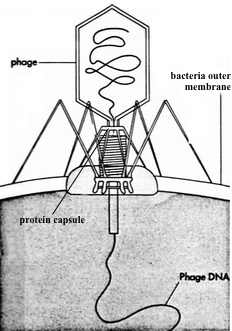
\includegraphics[width=0.42\textwidth]{figure1.png}
	\caption{A bacteriophage injecting its genome into a bacteria. The protein capsule both protects the 		genetic information while between hosts and pierces the membrane to allow injection. Adapted from Todar, 2012.}
\end{figure}

Once the genome has gained entry to the bacteria, the virus hijacks the machinery the host uses to replicate its own genome. In one mechanism of this, the virus incorporates its genome into the host genome, where it gets replicated and transported as the host cell reproduces. A different mechanism uses the host's ribosomes to synthesize proteins to promote virulence as well as new proteins to encapsulate new copies of the virus. Once there are many copies of the virus, they synthesize lysozyme, which breaks open the bacterial cell membrane, killing the host and allowing many new copies of the virus to escape and spread to nearby cells.

For the second mechanism, because the success of the virus means the death of the host, bacteria have evolved methods of resisting viruses. Coevolution has led to an arms race between viruses and bacteria, as they constantly find new ways to get around each other. This is especially evident in one model of virus-bacteria interaction known as gene-for-gene interaction. In these systems, the virus has a number of genes encoding virulence proteins that help it invade a cell and replicate its genome. Likewise, the bacteria has complementary resistance proteins that recognize and destroy the viral proteins. Through many generations, the viruses keep evolving new genes to get around the bacterial defenses, while the bacteria evolve to block resist the new genes. The progression of the genomes is cyclic, since selective pressure only acts on those loci where members of the bacteria population are still susceptible to the virus, and where the virus can still infect some bacteria. As the pressure lifts, specific resistance and virulence genes disappear from the population, since both host and parasite are prioritizing the genes most relevant to their interaction at that point in time (Person, 1959).

One interesting side-effect of this arms race is the relatively elevated mutation rate in many bacteria populations. In 2007, Pal et al. used a mixture of techniques to demonstrate that it was specifically coevolution with viruses that drove the increased mutation rate in susceptible bacteria. The mutation rate was mostly increased over time due to deleterious mutations in mismatch-repair genes, which code for proofreading proteins that normally check new copies of the bacterial genome for mutations and correct them. Without functioning mismatch-repair proteins, mutations are much more likely to passed on without being fixed. One of the tools Pal et al. used in their research was a genetic algorithm that simulated host-virus interactions, which they used specifically to model how mutation rates evolved over time. Their simulation behaved similarly to the predictions of the gene-for-gene model, with host mutation rate plateauing at the maximum allowed, while the frequencies individual genomes fluctuate over time as the selection pressure shifts in response to viral evolution (Figure 2) (Pal et al., 2007).

For our project, we attempted to replicate the simulation run by Pal et al., using a coevolution genetic algorithm. We based the representation of populations and fitness functions on those detailed by that paper. Unlike most GAs, we did not use crossover to introduce variability, because reproduction done in our model system is asexual, meaning there is only one parent for each child, and therefore no opportunity to undergo crossover. Besides complete replication, we also made some alterations to increase the similarity of our simulation to how the bacteria-virus system operates in nature. 

\begin{figure}[H]
	\centering
	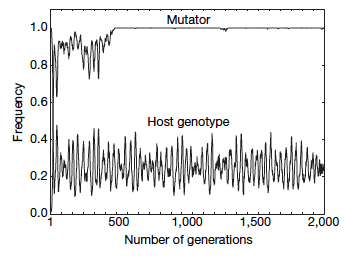
\includegraphics[width=0.6\textwidth]{figure2.png}
	\caption{Frequencies over time of a mutator gene that increases mutation rate 100-fold in the host population and one particular host genotype (Pal et al. 2007).}
\end{figure}

\section{Methods}
or Setup? 

What did we change from our inspiration?
\\- Allowing variable population with culls
\\- focused on gene-for-gene interaction
\\- soooo many fitnesses\\From paper, equation for host:
\begin{equation}
W_{H}(i,n) = (1-s_{v})^n(1-c)^z(1-s\cdot W_{Pij})
\end{equation}
Fitness for host $i$ with $n$ deleterious mutations infected by virus $j$, where $s_{v}$ is the effect of each deleterious mutation, $c$ is the cost of each resistance allele, $z$ is the number of resistance alleles, $s$ is maximum virulence of the virus, and $W_{Pij}$ is the fitness of virus $j$ on host $i$. Total fitness for each host is $\sum W_{H}(i,n)$ for all viruses able to infect it. Total fitness for each virus is $\sum W_{Pij}$ for each host it is able to infect. 

Equation for virus:
\begin{equation}
W_{Pij} = (1-p)^v
\end{equation}
where $p$ is the cost of virulence and $v$ is the number of virulence genes.

- table showing representation of each genome?
\\- how does selection work?
\\- mutation?
\\- flow chart!

\section{Results}
What are some things we've observed? graphs! How close did we come to what other paper saw? What are new things?

\section{Discussion}
What was hard? What was new? What are some new directions to try?

- interpreting their methods was interesting-- published for biologists! They didn't plan for people caring so much about their specific algorithm. 

\section{Works Cited}
Pal, C., M.D. Marcia, A. Oliver, I. Schachar, and A. Buckling. 2007. Coevolution with viruses drives the \\\-\hspace{0.75cm} evolution of bacterial mutation rates. Nature Letters. 450: 1079-1081.

Person, C. 1959. Gene-for-gene relationships in host:parasite systems. Canadian Journal of Botany. 37: \\\-\hspace{0.75cm} 1101- 1130.

Todar, K. 2012. Bacteriophage. Online Textbook of Bacteriology. Accessed 6.4.2015.\\\-\hspace{0.75cm} http://textbookofbacteriology.net/phage.html

\end{document}  